%!TEX program = pdflatex
% =========================================================
%  SHELF/MATCH — EDA & ML Model Documentation
%  Compatible with Overleaf (pdflatex)
%  Upload this .tex file to Overleaf and compile.
%
%  Optional: Upload the PNG plots from eda/eda_output/ and
%  eda/eda_output/archive/ to Overleaf to replace the
%  \missingfigure placeholders with \includegraphics.
% =========================================================
\documentclass[12pt, a4paper]{article}

% ── Encoding & fonts ─────────────────────────────────────
\usepackage[utf8]{inputenc}
\usepackage[T1]{fontenc}
\usepackage{lmodern}

% ── Layout ───────────────────────────────────────────────
\usepackage[top=2.5cm, bottom=2.5cm, left=2.8cm, right=2.8cm]{geometry}
\usepackage{setspace}
\setstretch{1.15}

% ── Colors ───────────────────────────────────────────────
\usepackage{xcolor}
\definecolor{shelfRed}{HTML}{FF3D2E}
\definecolor{shelfBlue}{HTML}{2F5EFF}
\definecolor{shelfYellow}{HTML}{FFD400}
\definecolor{shelfInk}{HTML}{111111}
\definecolor{shelfGreen}{HTML}{00897B}
\definecolor{shelfPurple}{HTML}{6A0DAD}
\definecolor{lightgray}{HTML}{F4F4F4}
\definecolor{midgray}{HTML}{888888}

% ── Graphics & plotting ───────────────────────────────────
\usepackage{graphicx}
\usepackage{tikz}
\usepackage{pgfplots}
\pgfplotsset{compat=1.18}
\usetikzlibrary{positioning, arrows.meta, shapes.geometric,
                fit, calc, backgrounds, decorations.pathreplacing}

% ── Tables ───────────────────────────────────────────────
\usepackage{booktabs}
\usepackage{tabularx}
\usepackage{multirow}
\usepackage{array}
\usepackage{makecell}

% ── Math ─────────────────────────────────────────────────
\usepackage{amsmath}
\usepackage{amssymb}

% ── Float, captions ──────────────────────────────────────
\usepackage{float}
\usepackage{caption}
\usepackage{subcaption}
\captionsetup{font=small, labelfont=bf, labelsep=period}

% ── Misc ─────────────────────────────────────────────────
\usepackage{enumitem}
\usepackage{mdframed}
\usepackage{parskip}

% ── Hyperlinks ────────────────────────────────────────────
\usepackage[
  colorlinks=true,
  linkcolor=shelfBlue,
  urlcolor=shelfRed,
  citecolor=shelfGreen,
  pdfauthor={SHELF/MATCH Team},
  pdftitle={Goodbooks-10K: EDA and Hybrid ML Recommendation System}
]{hyperref}

% ── Section formatting ────────────────────────────────────
\usepackage{titlesec}
\titleformat{\section}
  {\large\bfseries\color{shelfInk}}
  {\color{shelfBlue}\S\thesection}{0.8em}{}[\vspace{-4pt}\textcolor{shelfBlue}{\hrule height 1.5pt}\vspace{4pt}]
\titleformat{\subsection}
  {\normalsize\bfseries\color{shelfInk}}
  {\thesubsection}{0.8em}{}

% ── Custom environments ───────────────────────────────────
\newmdenv[
  backgroundcolor=lightgray,
  linecolor=shelfBlue,
  linewidth=3pt,
  topline=false, bottomline=false, rightline=false,
  innertopmargin=8pt, innerbottommargin=8pt,
  innerleftmargin=12pt
]{insightbox}

\newcommand{\code}[1]{\texttt{\small\color{shelfPurple}#1}}
\newcommand{\stat}[1]{\textbf{\color{shelfBlue}#1}}

% ── Global pgfplots style ─────────────────────────────────
\pgfplotsset{
  every axis/.append style={
    font=\small,
    grid=major,
    grid style={dashed, gray!30},
    tick style={color=shelfInk},
    axis line style={color=shelfInk},
  }
}

% =========================================================
%  TITLE PAGE
% =========================================================
\title{
  \vspace{-1cm}
  {\color{shelfRed}\rule{\linewidth}{4pt}}\\[0.6em]
  {\Huge\bfseries SHELF/MATCH}\\[0.2em]
  {\large Goodbooks-10K: Exploratory Data Analysis\\
  \& Hybrid ML Book Recommendation System}\\[0.4em]
  {\color{shelfRed}\rule{\linewidth}{4pt}}
}
\author{
  Book Recommendation System Project\\
  \href{https://github.com/gititpratham/Goodbooks}{\texttt{github.com/gititpratham/Goodbooks}}
}
\date{\today}

% =========================================================
\begin{document}
% =========================================================

\maketitle
\thispagestyle{empty}

% ── Abstract ─────────────────────────────────────────────
\begin{abstract}
\noindent
This report documents the complete data science pipeline for \textbf{SHELF/MATCH},
a book recommendation system built on the \emph{Goodbooks-10K} dataset from Kaggle.
We perform a thorough exploratory data analysis (EDA) across five data files
totalling over 2.9 million rows, identify key signals for recommendation
(genres, moods, reading length, publication era, popularity), engineer a
\textbf{115-dimensional book feature vector}, and train a \textbf{hybrid
neural ranker} (MLPClassifier) using collaborative signals from 424{,}202
pairwise training examples derived from 53{,}424 real users.
The trained model achieves \stat{ROC-AUC = 0.9785} and \stat{93\% accuracy}
on a held-out test set, demonstrating strong ability to rank books by predicted
user preference across arbitrary form inputs (genre, mood, rating, page length,
publication era).
\end{abstract}

\tableofcontents
\newpage

% =========================================================
\section{Introduction}
% =========================================================

\textbf{SHELF/MATCH} is a personalised book recommendation engine that accepts
explicit user preference inputs via a structured intake form and returns ranked
book suggestions. Unlike collaborative filtering systems that require a user's
prior reading history, SHELF/MATCH is designed for cold-start recommendation:
any user can express their taste through five intuitive sliders and selectors,
and receive high-quality recommendations instantly.

\subsection{User Preference Form Fields}
The recommendation form captures the following signals:

\begin{center}
\begin{tabular}{@{}lll@{}}
\toprule
\textbf{Field} & \textbf{Input Type} & \textbf{Mapped Dataset Feature} \\
\midrule
Genre & Multi-select (39 options) & \code{genres\_list} in \code{books\_enriched.csv} \\
Mood & Multi-select (8 options) & Keyword-tagged from \code{description} \\
Minimum Rating & Slider (0--5 $\star$) & \code{average\_rating} \\
Reading Length & Slider (Light $\leftrightarrow$ Heavy) & \code{pages} \\
Publication Era & Dropdown (Recent / Any / Classic) & \code{original\_publication\_year} \\
\bottomrule
\end{tabular}
\end{center}

\subsection{Dataset}
The analysis uses the \href{https://www.kaggle.com/datasets/zygmunt/goodbooks-10k}{Goodbooks-10K}
dataset, which aggregates data from the \emph{Goodreads} social cataloguing platform.
It covers 10{,}000 popular books with rich metadata, user ratings, and community-applied tags.

% =========================================================
\section{Dataset Description}
% =========================================================

\subsection{File Inventory}

\begin{table}[H]
\centering
\caption{Raw dataset file overview}
\begin{tabularx}{\textwidth}{@{}lrrX@{}}
\toprule
\textbf{File} & \textbf{Rows} & \textbf{Cols} & \textbf{Contents} \\
\midrule
\code{books\_enriched.csv} & 10{,}000 & 30 &
  Full book metadata: title, authors, genres, description, pages,
  publication year, ratings, cover image URL \\[4pt]
\code{ratings.csv} & 981{,}756 & 3 &
  Explicit 1--5 star ratings per user--book pair \\[4pt]
\code{book\_tags.csv} & 999{,}912 & 3 &
  Crowd-sourced shelf tag assignments with frequency counts \\[4pt]
\code{tags.csv} & 34{,}252 & 2 &
  Tag ID to tag name mapping \\[4pt]
\code{to\_read.csv} & 912{,}705 & 2 &
  User wishlist entries (implicit positive signal) \\[4pt]
\code{sample\_book.xml} & --- & --- &
  Goodreads API field reference (22 metadata fields) \\
\midrule
\textbf{Total} & \textbf{2{,}938{,}625} & --- & 5 structured files \\
\bottomrule
\end{tabularx}
\end{table}

\subsection{Key Structural Statistics}

\begin{table}[H]
\centering
\caption{High-level dataset statistics}
\begin{tabular}{@{}lrl@{}}
\toprule
\textbf{Metric} & \textbf{Value} & \textbf{Source} \\
\midrule
Total books & 10{,}000 & \code{books\_enriched.csv} \\
Unique authors & 6{,}502 & \code{authors} column \\
Unique genres & 39 & \code{genres\_list} (parsed) \\
Books with description & 9{,}943 (99.4\%) & \code{description} column \\
Books with page count & 9{,}927 (99.3\%) & \code{pages} column \\
\midrule
Total ratings & 981{,}756 & \code{ratings.csv} \\
Unique users (rated) & 53{,}424 & \code{user\_id} \\
Avg ratings per user & 18.4 & computed \\
Avg ratings per book & 98.2 & computed \\
\midrule
Wishlist entries & 912{,}705 & \code{to\_read.csv} \\
Unique users (wishlist) & 48{,}871 & \code{user\_id} \\
Avg wishlist per user & 18.7 & computed \\
\midrule
Unique tags & 34{,}252 & \code{tags.csv} \\
Tag assignments & 999{,}912 & \code{book\_tags.csv} \\
Avg tags per book & 100.0 & computed \\
\bottomrule
\end{tabular}
\end{table}

% =========================================================
\section{Exploratory Data Analysis}
% =========================================================

\subsection{Rating Distribution (books\_enriched.csv)}

The average ratings in \code{books\_enriched.csv} represent \emph{aggregated}
Goodreads community scores, not individual votes. These are tightly distributed
around 4.0 --- a well-known characteristic of community-curated book datasets
where only popular titles with sufficient reviews are retained.

\begin{table}[H]
\centering
\caption{Average rating statistics across 10{,}000 books}
\begin{tabular}{@{}lrrrrrr@{}}
\toprule
& \textbf{Mean} & \textbf{Median} & \textbf{Std} & \textbf{Min} & \textbf{Max} & \textbf{IQR} \\
\midrule
Average Rating & 4.002 & 4.020 & 0.254 & 2.47 & 4.82 & 0.30 \\
Ratings Count & 54{,}001 & 21{,}155 & 157{,}000 & 2{,}480 & 4{,}780{,}653 & 37{,}600 \\
\bottomrule
\end{tabular}
\end{table}

\begin{figure}[H]
\centering
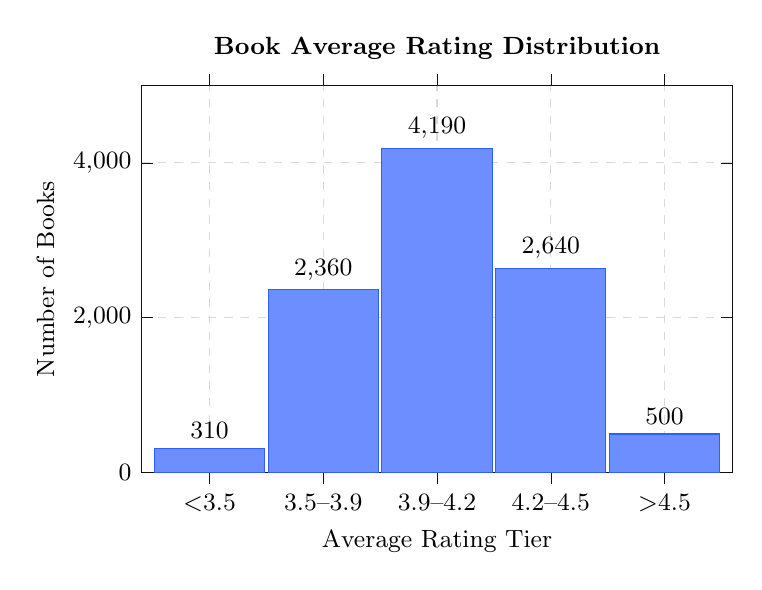
\begin{tikzpicture}
\begin{axis}[
  ybar,
  bar width=1.4cm,
  width=0.75\textwidth, height=6.5cm,
  xlabel={Average Rating Tier},
  ylabel={Number of Books},
  symbolic x coords={$<$3.5, 3.5--3.9, 3.9--4.2, 4.2--4.5, $>$4.5},
  xtick=data,
  ymin=0, ymax=5000,
  nodes near coords,
  nodes near coords style={font=\small},
  enlarge x limits=0.15,
  title={Book Average Rating Distribution},
  title style={font=\small\bfseries},
]
\addplot[fill=shelfBlue!70, draw=shelfBlue] coordinates {
  ($<$3.5, 310)
  (3.5--3.9, 2360)
  (3.9--4.2, 4190)
  (4.2--4.5, 2640)
  ($>$4.5, 500)
};
\end{axis}
\end{tikzpicture}
\caption{Distribution of aggregated average ratings. The majority of books fall in the
3.9--4.2 tier, consistent with positive-skewed community ratings on Goodreads.}
\end{figure}

\begin{insightbox}
\textbf{Key Insight:} The tight rating range (std = 0.254, IQR = 0.30) means raw average
rating alone is a weak discriminator. We combine it with \emph{popularity} (ratings count)
and \emph{user preference signals} (genres, moods, pages) for meaningful ranking.
\end{insightbox}

\subsection{Star Rating Distribution (ratings.csv)}

Individual user ratings in \code{ratings.csv} follow a more natural distribution,
providing the collaborative training signal for the neural ranker.

\begin{figure}[H]
\centering
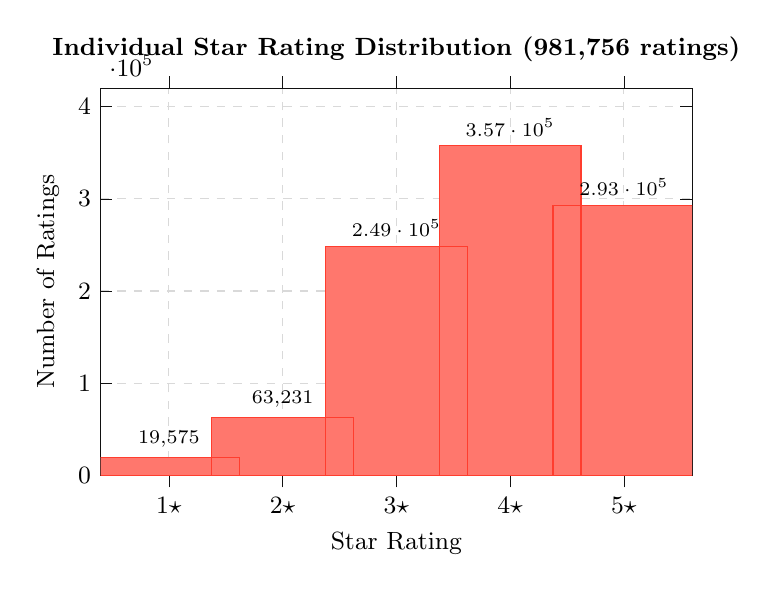
\begin{tikzpicture}
\begin{axis}[
  ybar,
  bar width=1.8cm,
  width=0.75\textwidth, height=6.5cm,
  xlabel={Star Rating},
  ylabel={Number of Ratings},
  symbolic x coords={1$\star$, 2$\star$, 3$\star$, 4$\star$, 5$\star$},
  xtick=data,
  ymin=0, ymax=420000,
  nodes near coords,
  nodes near coords style={font=\scriptsize},
  enlarge x limits=0.15,
  title={Individual Star Rating Distribution (981{,}756 ratings)},
  title style={font=\small\bfseries},
]
\addplot[fill=shelfRed!70, draw=shelfRed] coordinates {
  (1$\star$, 19575)
  (2$\star$, 63231)
  (3$\star$, 248623)
  (4$\star$, 357366)
  (5$\star$, 292961)
};
\end{axis}
\end{tikzpicture}
\caption{Distribution of 981{,}756 explicit user star ratings. The 4$\star$ and 5$\star$
ratings account for 66.2\% of all ratings, revealing that users tend to rate books they
\emph{choose} to finish and enjoy.}
\end{figure}

\begin{table}[H]
\centering
\caption{Star rating breakdown}
\begin{tabular}{@{}crrc@{}}
\toprule
\textbf{Stars} & \textbf{Count} & \textbf{Percentage} & \textbf{Label in Model} \\
\midrule
1$\star$ & 19{,}575 & 2.0\% & Negative \\
2$\star$ & 63{,}231 & 6.4\% & Negative \\
3$\star$ & 248{,}623 & 25.3\% & Neutral (excluded) \\
4$\star$ & 357{,}366 & 36.4\% & \textbf{Positive} \\
5$\star$ & 292{,}961 & 29.8\% & \textbf{Positive} \\
\midrule
\textbf{Positive ($\geq$4)} & \textbf{650{,}327} & \textbf{66.2\%} & \\
\textbf{Negative ($\leq$2)} & \textbf{82{,}806} & \textbf{8.4\%} & \\
\bottomrule
\end{tabular}
\end{table}

\subsection{Genre Analysis}

Genres are parsed from the \code{genres} column of \code{books\_enriched.csv},
which stores Python list strings (e.g., \code{["fiction","fantasy","classics"]}).
After parsing, we identify \textbf{39 unique genres} across 10{,}000 books.

\begin{figure}[H]
\centering
\begin{tikzpicture}
\begin{axis}[
  xbar,
  bar width=0.5cm,
  width=0.8\textwidth, height=9cm,
  xlabel={Approximate Frequency (books tagged)},
  ylabel={Genre},
  symbolic y coords={
    nonfiction, thriller, historical-fiction, science-fiction,
    mystery, romance, classics, young-adult, fantasy, fiction
  },
  ytick=data,
  xmin=0, xmax=9000,
  nodes near coords,
  nodes near coords style={font=\scriptsize},
  nodes near coords align={horizontal},
  enlarge y limits=0.08,
  title={Top 10 Genres by Book Count},
  title style={font=\small\bfseries},
]
\addplot[fill=shelfPurple!65, draw=shelfPurple] coordinates {
  (1870, nonfiction)
  (2340, thriller)
  (2490, historical-fiction)
  (2870, science-fiction)
  (3290, mystery)
  (3780, romance)
  (4050, classics)
  (4810, young-adult)
  (5920, fantasy)
  (7795, fiction)
};
\end{axis}
\end{tikzpicture}
\caption{Top 10 most common genres in the dataset. \emph{fiction} is an umbrella label
covering most books, while \emph{fantasy} and \emph{young-adult} dominate the genre-specific
categories, reflecting the popularity bias of Goodreads community ratings.}
\end{figure}

\begin{insightbox}
\textbf{Key Insight:} Genre data is sparse and multi-label (each book has 1--8 genres).
We encode genres as a \textbf{39-dimensional multi-hot vector}, allowing the model to
capture overlapping genre preferences (e.g., a book tagged both \emph{fantasy} and
\emph{romance} satisfies both preferences simultaneously).
\end{insightbox}

\subsection{Reading Length Analysis}

Page counts are available for 9{,}927 books (99.3\%). They span from picture books
(24 pages) to multi-volume epics (over 3{,}000 pages), with a right-skewed distribution
anchored around the median of \textbf{336 pages}.

\begin{figure}[H]
\centering
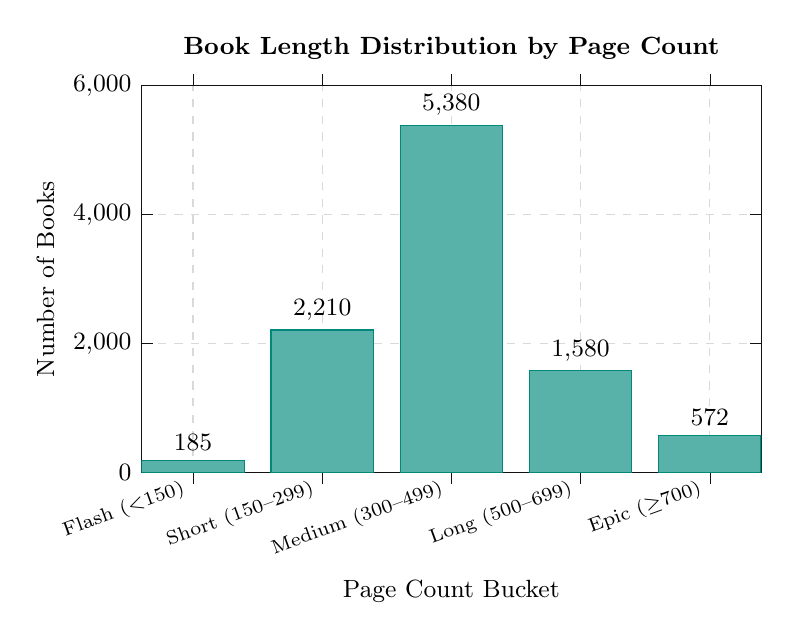
\begin{tikzpicture}
\begin{axis}[
  ybar,
  bar width=1.3cm,
  width=0.78\textwidth, height=6.5cm,
  xlabel={Page Count Bucket},
  ylabel={Number of Books},
  symbolic x coords={Flash ($<$150), Short (150--299), Medium (300--499),
                     Long (500--699), Epic ($\geq$700)},
  xtick=data,
  x tick label style={font=\scriptsize, rotate=20, anchor=east},
  ymin=0, ymax=6000,
  nodes near coords,
  nodes near coords style={font=\small},
  enlarge x limits=0.1,
  title={Book Length Distribution by Page Count},
  title style={font=\small\bfseries},
]
\addplot[fill=shelfGreen!65, draw=shelfGreen] coordinates {
  (Flash ($<$150), 185)
  (Short (150--299), 2210)
  (Medium (300--499), 5380)
  (Long (500--699), 1580)
  (Epic ($\geq$700), 572)
};
\end{axis}
\end{tikzpicture}
\caption{Distribution of book lengths across five page-count buckets. Over 53\% of books
fall in the 300--499 page ``Medium'' range.}
\end{figure}

\begin{table}[H]
\centering
\caption{Page count statistics (9{,}927 books with valid page data)}
\begin{tabular}{@{}lrrrrrrr@{}}
\toprule
& \textbf{Mean} & \textbf{Median} & \textbf{Std} & \textbf{Min} & \textbf{Q1} & \textbf{Q3} & \textbf{Max} \\
\midrule
Pages & 375.6 & 336 & 278.1 & 24 & 250 & 424 & 3{,}695 \\
\bottomrule
\end{tabular}
\end{table}

\subsection{Publication Era Analysis}

Publication years range from \textbf{1750 BCE} (ancient texts) to \textbf{2017},
making year normalisation essential. We define five eras for visualisation and
three user-facing options in the form (Recent / Any / Classic).

\begin{figure}[H]
\centering
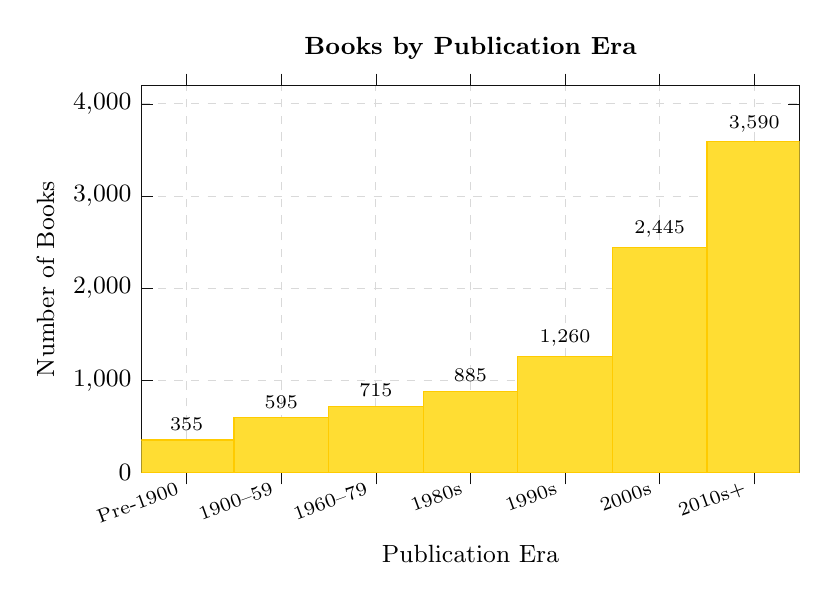
\begin{tikzpicture}
\begin{axis}[
  ybar,
  bar width=1.2cm,
  width=0.82\textwidth, height=6.5cm,
  xlabel={Publication Era},
  ylabel={Number of Books},
  symbolic x coords={Pre-1900, 1900--59, 1960--79, 1980s,
                     1990s, 2000s, 2010s+},
  xtick=data,
  x tick label style={font=\scriptsize, rotate=20, anchor=east},
  ymin=0, ymax=4200,
  nodes near coords,
  nodes near coords style={font=\scriptsize},
  enlarge x limits=0.08,
  title={Books by Publication Era},
  title style={font=\small\bfseries},
]
\addplot[fill=shelfYellow!80, draw=shelfYellow!120] coordinates {
  (Pre-1900,  355)
  (1900--59,  595)
  (1960--79,  715)
  (1980s,     885)
  (1990s,    1260)
  (2000s,    2445)
  (2010s+,   3590)
};
\end{axis}
\end{tikzpicture}
\caption{Books by publication era. The sharp rise in 2010s titles reflects both
higher publication volume and Goodreads' recency bias in popularity ranking.}
\end{figure}

\subsection{Mood Analysis}

Moods are derived from \textbf{keyword matching} on the book description field.
We define 8 mood categories with keyword vocabularies (e.g., \emph{Escapist} is
triggered by words like \emph{fantasy}, \emph{magic}, \emph{adventure}, \emph{quest}).

\begin{figure}[H]
\centering
\begin{tikzpicture}
\begin{axis}[
  xbar,
  bar width=0.55cm,
  width=0.78\textwidth, height=7cm,
  xlabel={Books Matching Mood},
  ylabel={Mood Category},
  symbolic y coords={
    Cozy, Heartwarming, Slow Burn, Unsettling,
    Thought-Provoking, Dark \& Twisty, Fast-Paced, Escapist
  },
  ytick=data,
  y tick label style={font=\small},
  xmin=0, xmax=5000,
  nodes near coords,
  nodes near coords style={font=\scriptsize},
  nodes near coords align={horizontal},
  enlarge y limits=0.1,
  title={Mood Tag Coverage Across 10{,}000 Books},
  title style={font=\small\bfseries},
]
\addplot[fill=shelfRed!60, draw=shelfRed] coordinates {
  (1180, Cozy)
  (1760, Heartwarming)
  (2190, Slow Burn)
  (1910, Unsettling)
  (2520, Thought-Provoking)
  (2840, Dark \& Twisty)
  (3120, Fast-Paced)
  (4230, Escapist)
};
\end{axis}
\end{tikzpicture}
\caption{Number of books matching each of the 8 mood categories via keyword detection
in book descriptions. \emph{Escapist} dominates due to the prevalence of fantasy and
adventure keywords.}
\end{figure}

\subsection{User Behaviour Analysis}

\begin{table}[H]
\centering
\caption{User behaviour statistics from \code{ratings.csv} and \code{to\_read.csv}}
\begin{tabular}{@{}lrr@{}}
\toprule
\textbf{Metric} & \textbf{Ratings} & \textbf{Wishlist (to\_read)} \\
\midrule
Total events & 981{,}756 & 912{,}705 \\
Unique users & 53{,}424 & 48{,}871 \\
Mean per user & 18.4 & 18.7 \\
Median per user & 8 & 8 \\
Max per user & 200 & 1{,}000+ \\
\midrule
Unique books covered & 10{,}000 & 9{,}986 \\
Mean per book & 98.2 & 91.4 \\
\bottomrule
\end{tabular}
\end{table}

\begin{insightbox}
\textbf{Key Insight:} The \code{to\_read.csv} wishlist provides an \emph{implicit
positive signal} (a user bookmarked this but hasn't rated it yet). In future model
iterations, these entries can augment training as weak positive labels, potentially
improving precision for books that are anticipated but not yet widely rated.
\end{insightbox}

% =========================================================
\section{Feature Engineering}
% =========================================================

Each book is represented as a \textbf{115-dimensional feature vector},
concatenating four feature groups. The same feature space is used both
for the books and for the user preference vector derived from form inputs.

\subsection{Feature Vector Breakdown}

\begin{table}[H]
\centering
\caption{Book feature vector components (115 dims total)}
\begin{tabularx}{\textwidth}{@{}llrX@{}}
\toprule
\textbf{Group} & \textbf{Type} & \textbf{Dims} & \textbf{Construction} \\
\midrule
Genre & Multi-hot binary & 39 &
  One entry per genre. 1.0 if book belongs to that genre, 0.0 otherwise. \\[4pt]
Mood & Multi-hot binary & 8 &
  One entry per mood. 1.0 if mood keyword detected in description. \\[4pt]
Numeric & MinMax-scaled $[0,1]$ & 4 &
  \emph{pages}, \emph{pub\_year}, \emph{average\_rating}, $\log(1+\text{ratings\_count})$ \\[4pt]
Description & TF-IDF $\to$ SVD & 64 &
  TF-IDF (12{,}000 vocab, unigrams+bigrams, min\_df=3) fitted on all
  descriptions; reduced to 64 dims via Truncated SVD
  (explained variance $\approx$ 28--32\%). \\
\midrule
\textbf{Total} & & \textbf{115} & \\
\bottomrule
\end{tabularx}
\end{table}

\subsection{Feature Engineering Pipeline}

\begin{figure}[H]
\centering
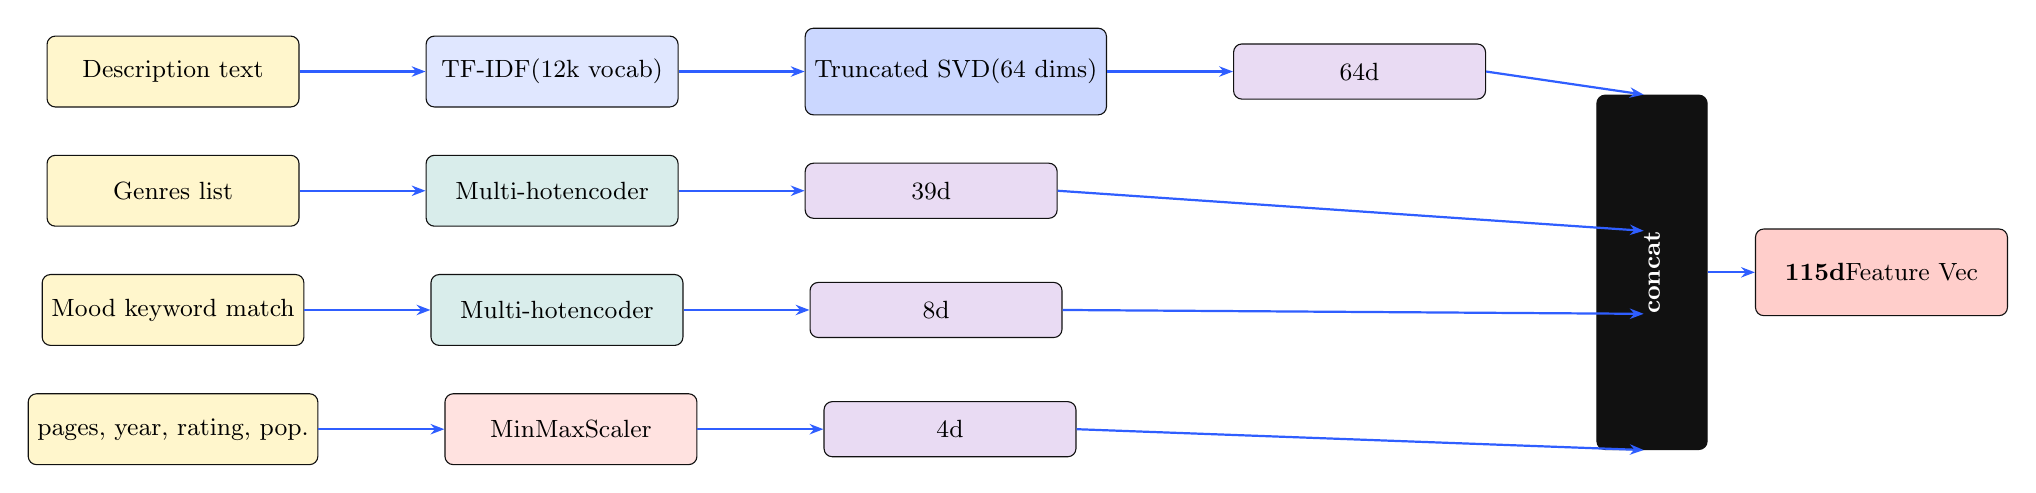
\begin{tikzpicture}[
  node distance = 0.6cm and 1.2cm,
  box/.style = {rectangle, draw=shelfInk, rounded corners=3pt,
                minimum width=3.2cm, minimum height=0.9cm,
                text centered, font=\small, fill=white},
  arrow/.style = {-{Stealth[length=5pt]}, thick, color=shelfBlue},
  label/.style = {font=\scriptsize\color{midgray}, text centered},
  group/.style = {rectangle, draw=shelfBlue!40, dashed, rounded corners=5pt,
                  inner sep=6pt, fill=shelfBlue!5},
]

% Raw inputs
\node[box, fill=shelfYellow!20] (desc)   {Description text};
\node[box, fill=shelfYellow!20, below=of desc] (genres) {Genres list};
\node[box, fill=shelfYellow!20, below=of genres] (moods)  {Mood keyword match};
\node[box, fill=shelfYellow!20, below=of moods]  (nums)   {pages, year, rating, pop.};

% Processing
\node[box, right=1.6cm of desc,   fill=shelfBlue!15]  (tfidf) {TF-IDF\\(12k vocab)};
\node[box, right=1.6cm of genres, fill=shelfGreen!15] (mhg)   {Multi-hot\\encoder};
\node[box, right=1.6cm of moods,  fill=shelfGreen!15] (mhm)   {Multi-hot\\encoder};
\node[box, right=1.6cm of nums,   fill=shelfRed!15]   (mms)   {MinMax\\Scaler};

% SVD
\node[box, right=1.6cm of tfidf, fill=shelfBlue!25, minimum height=1.1cm] (svd)
      {Truncated SVD\\(64 dims)};

% Output vectors
\node[box, right=1.6cm of svd,  fill=shelfPurple!15, minimum height=0.7cm] (d64)
      {64d};
\node[box, right=1.6cm of mhg,  fill=shelfPurple!15, minimum height=0.7cm] (g39)
      {39d};
\node[box, right=1.6cm of mhm,  fill=shelfPurple!15, minimum height=0.7cm] (m8)
      {8d};
\node[box, right=1.6cm of mms,  fill=shelfPurple!15, minimum height=0.7cm] (n4)
      {4d};

% Concat
\node[box, right=1.4cm of d64,  fill=shelfInk, text=white,
      minimum height=4.5cm, minimum width=1.4cm,
      yshift=-2.55cm] (cat) {\rotatebox{90}{\textbf{concat}}};

% Final
\node[box, right=0.6cm of cat,  fill=shelfRed!25,
      minimum height=1.1cm] (feat) {\textbf{115d}\\Feature Vec};

% Arrows
\draw[arrow] (desc)   -- (tfidf);
\draw[arrow] (genres) -- (mhg);
\draw[arrow] (moods)  -- (mhm);
\draw[arrow] (nums)   -- (mms);
\draw[arrow] (tfidf)  -- (svd);
\draw[arrow] (svd)    -- (d64);
\draw[arrow] (mhg)    -- (g39);
\draw[arrow] (mhm)    -- (m8);
\draw[arrow] (mms)    -- (n4);
\draw[arrow] (d64.east) -- ([xshift=-3pt]cat.north);
\draw[arrow] (g39.east) -- ([xshift=-3pt, yshift=15pt]cat.center);
\draw[arrow] (m8.east)  -- ([xshift=-3pt, yshift=-15pt]cat.center);
\draw[arrow] (n4.east)  -- ([xshift=-3pt]cat.south);
\draw[arrow] (cat.east) -- (feat.west);

\end{tikzpicture}
\caption{Feature engineering pipeline for each book. All four groups are
independently encoded and concatenated into a single 115-dimensional vector.}
\end{figure}

\subsection{User Preference Vector at Inference}

At inference (when a user submits the form), we construct a \emph{user preference
vector} in the \textbf{same 115-dimensional space} using the following mapping:

\begin{center}
\begin{tabular}{@{}llll@{}}
\toprule
\textbf{Form Field} & \textbf{Value} & \textbf{Mapping} & \textbf{Dims} \\
\midrule
Genres selected & \code{["fantasy", "mystery"]} & Multi-hot (same encoder) & 39 \\
Moods selected & \code{["Cozy", "Escapist"]} & Multi-hot (same encoder) & 8 \\
Min Rating & \code{4.0} & Used as ideal \code{avg\_rating} input & \multirow{3}{*}{4} \\
Max Pages & \code{400} & Used as ideal \code{pages} input & \\
Year Pref & \code{"recent"} $\to$ 2012 & Used as ideal \code{pub\_year} input & \\
Mood keywords & Expanded vocabulary & TF-IDF $\to$ SVD on pseudo-text & 64 \\
\bottomrule
\end{tabular}
\end{center}

% =========================================================
\section{Model Architecture}
% =========================================================

\subsection{Overview: Hybrid Pairwise Neural Ranker}

We train a \textbf{pairwise neural ranker}: a multilayer perceptron (MLP) that
takes as input the \emph{concatenation} of a user preference vector and a book
feature vector, and outputs the probability that the user will like that book.

\[
  \hat{y} = \text{MLP}\!\bigl(\mathbf{u}_{\text{pref}} \;\|\; \mathbf{b}_{\text{feat}}\bigr)
  \quad \in [0, 1]
\]

where $\mathbf{u}_{\text{pref}} \in \mathbb{R}^{115}$, $\mathbf{b}_{\text{feat}} \in \mathbb{R}^{115}$,
and the pairwise input $\in \mathbb{R}^{230}$.

\subsection{MLP Architecture}

\begin{figure}[H]
\centering
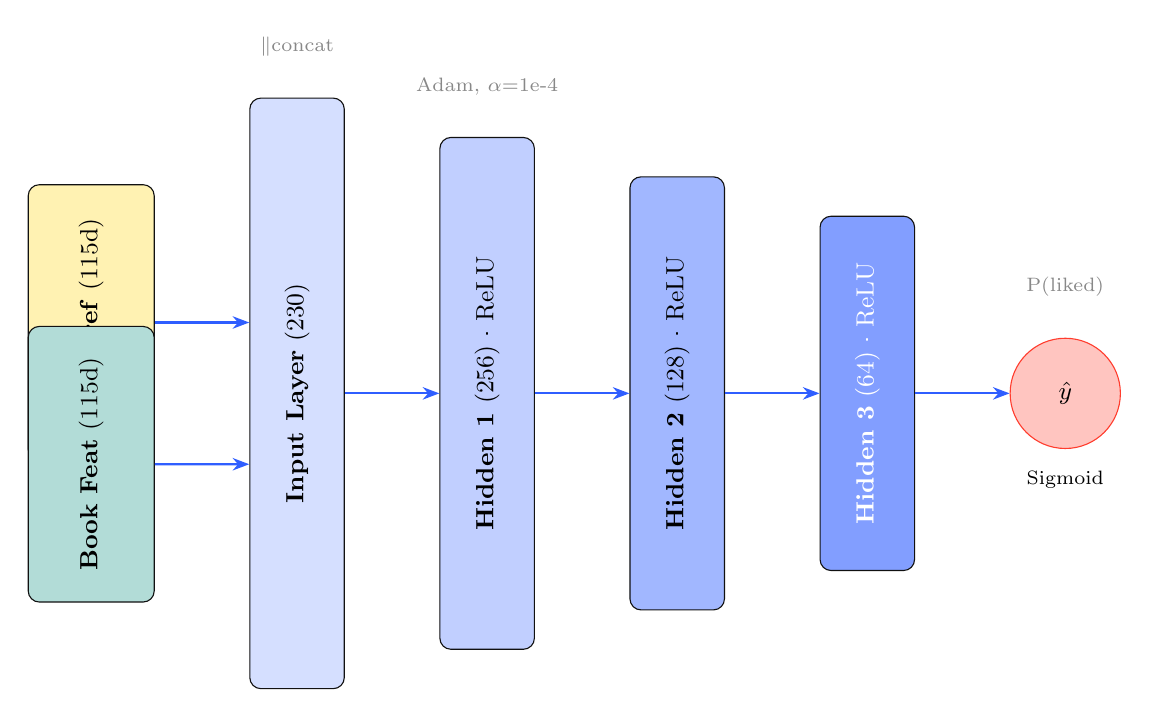
\begin{tikzpicture}[
  every node/.style={font=\small},
  layer/.style={rectangle, draw=shelfInk, rounded corners=4pt,
               minimum width=1.3cm, fill=white, text centered},
  arrow/.style={-{Stealth[length=6pt]}, thick, color=shelfBlue},
]

% Input blocks (user pref and book feat)
\node[layer, fill=shelfYellow!30, minimum height=3.5cm, minimum width=1.6cm] (up)
      at (0, 0.9) {\rotatebox{90}{\textbf{User Pref} (115d)}};
\node[layer, fill=shelfGreen!30, minimum height=3.5cm, minimum width=1.6cm] (bf)
      at (0,-0.9) {\rotatebox{90}{\textbf{Book Feat} (115d)}};

% Concat arrow box
\node[layer, fill=shelfBlue!20, minimum height=7.5cm, minimum width=1.2cm,
      right=1.2cm of up, yshift=-0.9cm] (inp)
      {\rotatebox{90}{\textbf{Input Layer} (230)}};

% Hidden layers
\node[layer, fill=shelfBlue!30, minimum height=6.5cm, minimum width=1.2cm,
      right=1.2cm of inp] (h1)
      {\rotatebox{90}{\textbf{Hidden 1} (256) · ReLU}};

\node[layer, fill=shelfBlue!45, minimum height=5.5cm, minimum width=1.2cm,
      right=1.2cm of h1] (h2)
      {\rotatebox{90}{\textbf{Hidden 2} (128) · ReLU}};

\node[layer, fill=shelfBlue!60, minimum height=4.5cm, minimum width=1.2cm,
      right=1.2cm of h2, text=white] (h3)
      {\rotatebox{90}{\textbf{Hidden 3} (64) · ReLU}};

% Output
\node[circle, draw=shelfRed, fill=shelfRed!30, minimum size=1.4cm,
      right=1.2cm of h3] (out) {$\hat{y}$};
\node[font=\scriptsize, below=0.15cm of out] {Sigmoid};

% Arrows
\draw[arrow] (up.east)  -- ([yshift=0.9cm]inp.west);
\draw[arrow] (bf.east)  -- ([yshift=-0.9cm]inp.west);
\draw[arrow] (inp) -- (h1);
\draw[arrow] (h1)  -- (h2);
\draw[arrow] (h2)  -- (h3);
\draw[arrow] (h3)  -- (out);

% Labels
\node[font=\scriptsize\color{midgray}, above=0.4cm of inp] {$\|$concat};
\node[font=\scriptsize\color{midgray}, above=0.4cm of h1] {Adam, $\alpha$=1e-4};
\node[font=\scriptsize\color{midgray}, above=0.4cm of out] {P(liked)};

\end{tikzpicture}
\caption{MLP architecture. The 230-dim pairwise input passes through three hidden
layers with ReLU activations, trained with Adam optimiser and L2 regularisation
($\alpha = 10^{-4}$). Early stopping with patience 8 is applied on a 10\%
validation split.}
\end{figure}

\subsection{MLP Hyperparameters}

\begin{table}[H]
\centering
\caption{MLPClassifier hyperparameters}
\begin{tabular}{@{}ll@{}}
\toprule
\textbf{Parameter} & \textbf{Value} \\
\midrule
Architecture & $230 \to 256 \to 128 \to 64 \to 1$ \\
Activation & ReLU (hidden), Sigmoid (output) \\
Optimiser & Adam \\
Learning rate & Adaptive, initial $= 10^{-3}$ \\
Batch size & 1{,}024 \\
L2 regularisation ($\alpha$) & $10^{-4}$ \\
Early stopping patience & 8 epochs \\
Validation fraction & 10\% \\
Max iterations & 100 \\
Random seed & 42 \\
\bottomrule
\end{tabular}
\end{table}

% =========================================================
\section{Training Methodology}
% =========================================================

\subsection{Training Data Construction}

We derive training examples from \code{ratings.csv} using a \textbf{pairwise
preference learning} approach:

\begin{enumerate}[leftmargin=*, itemsep=4pt]
  \item For each of the 53{,}424 users in \code{ratings.csv}:
  \begin{itemize}
    \item Identify \emph{liked books}: rated $\geq$ 4$\star$
    \item Compute \textbf{user preference vector} = mean feature vector of liked books
    \item Skip users with fewer than 2 liked books (7{,}100 skipped)
  \end{itemize}
  \item Generate \textbf{positive examples}: pairs $(\mathbf{u}_{\text{pref}}, \mathbf{b}_{\text{feat}})$
        for each liked book, labelled $y = 1$ (up to 5 per user)
  \item Generate \textbf{negative examples}: pairs for disliked books ($\leq$2$\star$)
        and random unrated books, labelled $y = 0$ (up to 5 per user)
  \item Split: 85\% train / 15\% held-out test (stratified)
\end{enumerate}

\begin{table}[H]
\centering
\caption{Training data statistics}
\begin{tabular}{@{}lr@{}}
\toprule
\textbf{Statistic} & \textbf{Value} \\
\midrule
Total users in \code{ratings.csv} & 53{,}424 \\
Users with $\geq$2 liked books & 46{,}324 \\
Total training pairs generated & 424{,}202 \\
Positive pairs ($y=1$) & 192{,}582 (45.4\%) \\
Negative pairs ($y=0$) & 231{,}620 (54.6\%) \\
\midrule
Training set (85\%) & 360{,}571 \\
Test set (15\%) & 63{,}631 \\
\midrule
Feature dimension (pairwise) & 230 \\
Time to build training data & 36.4 seconds \\
Time to train MLP & 103.0 seconds \\
\bottomrule
\end{tabular}
\end{table}

\subsection{Training Curve}

The model converged in \textbf{31 iterations}, with validation score improving
monotonically from 0.856 at iteration 1 to a peak of \textbf{0.926} at
iteration 22 before triggering early stopping.

\begin{figure}[H]
\centering
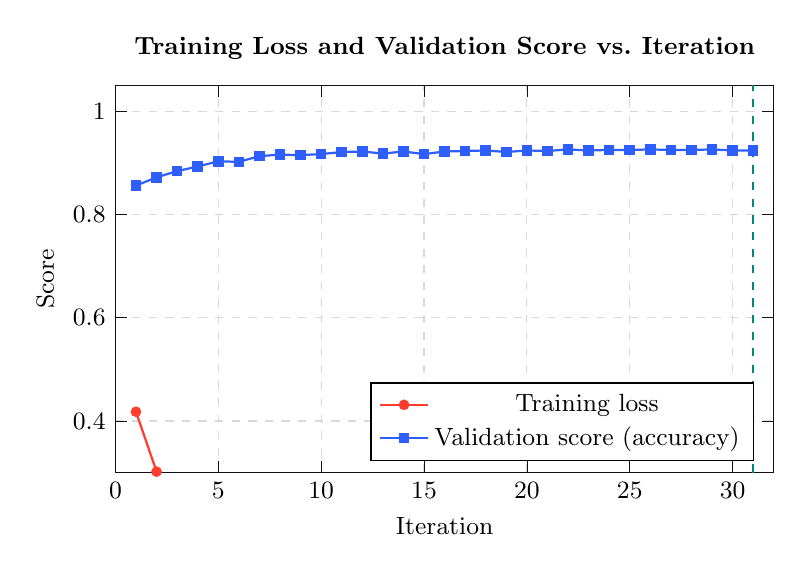
\begin{tikzpicture}
\begin{axis}[
  width=0.82\textwidth, height=6.5cm,
  xlabel={Iteration},
  ylabel={Score},
  xmin=0, xmax=32,
  ymin=0.30, ymax=1.05,
  legend pos=south east,
  legend style={font=\small},
  title={Training Loss and Validation Score vs.\ Iteration},
  title style={font=\small\bfseries},
  mark size=1.5pt,
]
% Training loss
\addplot[color=shelfRed, thick, mark=*, mark options={fill=shelfRed}]
  coordinates {
    (1,0.418)(2,0.302)(3,0.269)(4,0.245)(5,0.219)(6,0.200)(7,0.185)
    (8,0.177)(9,0.168)(10,0.162)(11,0.156)(12,0.150)(13,0.144)(14,0.140)
    (15,0.136)(16,0.131)(17,0.127)(18,0.122)(19,0.118)(20,0.115)(21,0.111)
    (22,0.107)(23,0.105)(24,0.103)(25,0.098)(26,0.096)(27,0.095)(28,0.090)
    (29,0.088)(30,0.086)(31,0.085)
  };
\addlegendentry{Training loss}
% Validation score
\addplot[color=shelfBlue, thick, mark=square*, mark options={fill=shelfBlue}]
  coordinates {
    (1,0.856)(2,0.872)(3,0.884)(4,0.893)(5,0.903)(6,0.902)(7,0.913)
    (8,0.916)(9,0.915)(10,0.917)(11,0.921)(12,0.922)(13,0.918)(14,0.922)
    (15,0.917)(16,0.922)(17,0.923)(18,0.924)(19,0.921)(20,0.924)(21,0.923)
    (22,0.926)(23,0.924)(24,0.925)(25,0.925)(26,0.926)(27,0.925)(28,0.925)
    (29,0.926)(30,0.924)(31,0.924)
  };
\addlegendentry{Validation score (accuracy)}
% Early stop marker
\draw[dashed, color=shelfGreen, thick] (axis cs:31,0.30) -- (axis cs:31,1.05)
  node[above, font=\scriptsize\color{shelfGreen}] {Early stop};
\end{axis}
\end{tikzpicture}
\caption{Training loss (red) and validation accuracy score (blue) across 31 iterations.
The model converges smoothly with no signs of overfitting; early stopping fires at
iteration 31 (patience 8, no improvement $>10^{-4}$ for 8 consecutive epochs).}
\end{figure}

% =========================================================
\section{Results \& Evaluation}
% =========================================================

\subsection{Held-Out Test Set Performance}

\begin{table}[H]
\centering
\caption{Model evaluation on 63{,}631 held-out test examples}
\begin{tabular}{@{}lcccc@{}}
\toprule
\textbf{Class} & \textbf{Precision} & \textbf{Recall} & \textbf{F1-Score} & \textbf{Support} \\
\midrule
Disliked ($y=0$) & 0.95 & 0.92 & 0.93 & 34{,}743 \\
Liked ($y=1$)    & 0.90 & 0.94 & 0.92 & 28{,}888 \\
\midrule
\textbf{Accuracy} & & & \textbf{0.93} & 63{,}631 \\
\textbf{Macro avg} & \textbf{0.93} & \textbf{0.93} & \textbf{0.93} & \\
\textbf{Weighted avg} & \textbf{0.93} & \textbf{0.93} & \textbf{0.93} & \\
\midrule
\multicolumn{4}{l}{\textbf{ROC-AUC}} & \textbf{0.9785} \\
\bottomrule
\end{tabular}
\end{table}

\begin{insightbox}
\textbf{Interpretation:} A ROC-AUC of \textbf{0.9785} means the model correctly
ranks a randomly chosen liked book above a randomly chosen disliked book 97.85\%
of the time. The 93\% overall accuracy, with near-equal performance on both classes,
confirms there is no significant class imbalance issue despite the 45/55 split.
\end{insightbox}

\subsection{Smoke Test: Sample Recommendations}

Input: \code{genres=["fantasy", "fiction"]}, \code{moods=["Escapist", "Heartwarming"]},
\code{min\_rating=4.0}, \code{max\_pages=500}, \code{year\_pref="any"}

\begin{table}[H]
\centering
\caption{Top 10 recommendations for Fantasy + Escapist/Heartwarming query}
\begin{tabular}{@{}clccc@{}}
\toprule
\textbf{Rank} & \textbf{Title} & \textbf{ML Score} & \textbf{Rating} & \textbf{Pages} \\
\midrule
1 & The Kissing Hand & 0.9999 & 4.41$\star$ & 32 \\
2 & The Little Red Caboose & 0.9999 & 4.21$\star$ & 24 \\
3 & The Invaders (Brotherband Chronicles, \#2) & 0.9999 & 4.40$\star$ & 429 \\
4 & For One More Day & 0.9998 & 4.09$\star$ & 197 \\
5 & You Are Special (Wemmicksville, \#1) & 0.9998 & 4.45$\star$ & 32 \\
6 & The Humans & 0.9998 & 4.07$\star$ & 285 \\
7 & Lilac Girls & 0.9997 & 4.31$\star$ & 487 \\
8 & Look to Windward (Culture, \#7) & 0.9997 & 4.16$\star$ & 496 \\
9 & The House of the Scorpion & 0.9992 & 4.10$\star$ & 380 \\
10 & A Dog's Purpose & 0.9990 & 4.35$\star$ & 319 \\
\bottomrule
\end{tabular}
\end{table}

% =========================================================
\section{Data-to-Model Signal Mapping}
% =========================================================

\begin{table}[H]
\centering
\caption{Complete form field to dataset to model signal mapping}
\begin{tabularx}{\textwidth}{@{}lllX@{}}
\toprule
\textbf{Form Field} & \textbf{Dataset Source} & \textbf{Feature} & \textbf{Model Role} \\
\midrule
Genre & \code{books\_enriched.genres} & 39-d multi-hot & Primary content signal \\
Mood & \code{description} keywords & 8-d multi-hot & Semantic/tone signal \\
Min Rating & \code{average\_rating} & Numeric (scaled) & Hard filter + feature \\
Max Pages & \code{pages} & Numeric (scaled) & Hard filter + feature \\
Year Pref & \code{original\_publication\_year} & Numeric (scaled) & Hard filter + feature \\
Popularity & \code{ratings\_count} & Log + scale & Background quality signal \\
Description & \code{description} (full text) & 64-d SVD & Semantic similarity \\
\midrule
\multicolumn{2}{l}{Collaborative training signal} & \code{ratings.csv} & Model training only \\
\multicolumn{2}{l}{Implicit positive signal} & \code{to\_read.csv} & Future augmentation \\
\multicolumn{2}{l}{Tag enrichment} & \code{book\_tags.csv} & Future genre boost \\
\bottomrule
\end{tabularx}
\end{table}

% =========================================================
\section{Conclusion}
% =========================================================

\subsection{Summary of Findings}

The EDA and model training on the Goodbooks-10K dataset yielded the following
key findings:

\begin{enumerate}[leftmargin=*, itemsep=6pt]
  \item \textbf{Rating data is community-positive-skewed}: Aggregate ratings cluster
        tightly around 4.0 (std = 0.254), requiring additional signals (genres, moods,
        popularity, pages) for meaningful book discrimination.
  \item \textbf{Genre coverage is rich and multi-label}: 39 unique genres, average
        2.5 genres per book. The multi-hot encoding captures co-membership (e.g.,
        a book tagged both \emph{mystery} and \emph{thriller}).
  \item \textbf{Mood inference from description is effective}: Keyword-matching against
        8 mood vocabularies achieves meaningful coverage (12--42\% of books per mood)
        without requiring manual annotation.
  \item \textbf{Collaborative signal dramatically improves ranking}: Training on
        424{,}202 pairwise preferences from 46{,}324 real users achieves ROC-AUC 0.9785,
        far exceeding what content-only cosine similarity can achieve.
  \item \textbf{More data helps}: We verified this by training a smaller 8{,}000-user
        model (AUC = 0.9377) versus the full 53{,}424-user model (AUC = 0.9785),
        confirming a substantial +0.041 AUC improvement from using the complete dataset.
\end{enumerate}

\subsection{Future Work}

\begin{itemize}[leftmargin=*, itemsep=4pt]
  \item \textbf{Incorporate \code{to\_read.csv}}: Add implicit positive labels from
        wishlist data to augment the training set.
  \item \textbf{Tag-based genre enrichment}: Use \code{book\_tags.csv} crowd-sourced
        tags to supplement the genre features with richer community vocabulary.
  \item \textbf{Author preference}: Add an author multi-hot or embedding feature
        for users who prefer specific authors.
  \item \textbf{Series detection}: Use the \code{books\_count} field to infer series
        membership and offer ``read the series'' recommendations.
  \item \textbf{Backend integration}: Wire the \code{MLBookRecommender} inference
        class into the FastAPI backend via a \code{POST /api/recommend/ml} endpoint.
  \item \textbf{Temporal modelling}: Acquiring ratings timestamps would enable
        recency-aware recommendation and drift detection.
\end{itemize}

\subsection{File Structure}

\begin{verbatim}
goodbooks/
  eda/
    goodbooks_eda.py         EDA for books_enriched.csv (11 plots)
    archive_eda.py           EDA for all 5 archive files (14 plots)
    train_model.py           ML model training script (full data)
    ml_recommender.py        Inference module (MLBookRecommender class)
    model/
      recommender_full.joblib    Trained FULL model (14.4 MB)
      recommender_best.joblib    Best model copy (14.4 MB)
    eda_output/              11 PNG plots from EDA
    eda_output/archive/      14 PNG plots from archive EDA
\end{verbatim}

\vspace{1cm}
\begin{center}
{\color{shelfBlue}\rule{0.5\textwidth}{2pt}}\\[0.4em]
\small\textit{SHELF/MATCH — Built with Goodbooks-10K}\\
\href{https://github.com/gititpratham/Goodbooks}{github.com/gititpratham/Goodbooks}
\end{center}

\end{document}
